\documentclass[a4paper,12pt,]{article}
\usepackage[utf8]{inputenc}

\title{Feature 2: Auswertung eines monatlichen Teamfragebogens}
\author{A.~Heckl, A.~Kohles, A.~Lehene, A.~Mütter}
\date{Februar 2020}

\usepackage[left=2.5cm,right=2.5cm,top=2.5cm,bottom=2.5cm]{geometry}
\usepackage{natbib}
\usepackage{graphicx}
\usepackage[ngerman]{babel}
\newcommand{\ToDo}[1]{
\begin{center}
\fbox{
\begin{minipage}{0.9\textwidth}
#1
\end{minipage}
}
\end{center}
}

\begin{document}

\maketitle
\begin{figure}
\begin{minipage}[b]{\textwidth}
\ToDo{\tiny\textbf{Hinweis:} Wir waren uns bei der Formulierung des Tagebuchs und des Abschlussberichts über die Richtlinien der gendergerechten Sprache und der gendergerechten Formulierung bewusst.
Aus Gründen der Übersichtlichkeit und der einfacheren Lesbarkeit haben wir uns entschieden darauf hinzuweisen, dass in diesem Dokument mit allen männlichen Formulierungen von Personen (Angestellter, Mitarbeiter, Vorgesetzter) selbstverständlich auch die weiblichen Pendants gemeint sind, und diese in keiner Weise vernachlässigbar oder weniger bedeutungsvoll sind.}
\end{minipage}
\end{figure}

\section{Deskriptive Systembeschreibung}

Die Stimmung in unserem Arbeitsteam ist verbesserungsfähig. Dies macht sich bemerkbar in sinkenden Produktivitätsraten und abnehmender Qualität der teaminternen Kommunikation. Zur Verbesserung dieser Umstände soll die Teamstimmung erfasst werden, um Angriffspunkte für Verbesserungsmaßnahmen zu erkennen.
Hierfür wurde vom Arbeitgeber in Kooperation mit dem Betriebsrat ein Fragebogen ausgearbeitet, welcher die Arbeitnehmer regelmäßig zu Umfragen bezüglich der Stimmung im Team, zur vorherrschenden Meinung über den Vorgesetzten und zu eventuell vorhandener Kritik befragt. Die Fragen stammen aus dem „Fragebogen zur Qualität unserer Teamarbeit“ vom Institut für Psychologietransfer in Bamberg,\footnote{\tt https://www.ipt-bamberg.de/unternehmen/downloads.html} wobei ähnliche Fragen zusammengefasst oder weggelassen wurden, um auf 12 Fragen für das Plugin zu kommen. Die Fragen, die den Vorgesetzen bzw. den Manager betreffen, sollen hierbei mit dessen Selbsteinschätzung verglichen werden, um so Diskrepanzen zwischen dem Team und der Führungskraft zu entdecken. Um problembereitende Mitarbeiter aufzuspüren, soll zudem in jeder dieser monatlichen Umfragen ein Mitarbeiter des Teams in den Fokus genommen werden, zu welchem individuelle Fragen im Fragebogen gestellt werden. Damit hat jeder Mitarbeiter die Möglichkeit  individuelles Feedback zu erhalten.
Neben den 12 Fragen aus dem Fragebogen gibt es noch eine allgemeine Bewertungsskala der Teamstimmung von 1-10, sowie die Möglichkeit zu Eingabe von Freitext.
Die Ergebnisse sollen grafisch aufbereitet werden, um dem Team die Entwicklung der Stimmung zu zeigen, und gegebenenfalls Fortschritte oder Verschlechterungen zu visualisieren. Der in den Fokus der Umfrage genommene Angestellte erhält zudem ein individuelles Bewertungszeugnis, welches er mit seinem Vorgesetzten diskutiert und gegebenenfalls persönliche oder berufliche Konsequenzen zur Folge hat (Beförderung, Aufruf zu mehr Kooperation, Versetzung, …).
Die Unterschiede zwischen der Teameinschätzung und der Einschätzung des Managers werden ebenfalls ermittelt, um eventuelle Diskrepanzen bei Teamsitzungen diskutieren zu können.

\section{Wertekonflikte}

\subsection{Fragestellungen}
Vor der Umsetzung einer solchen Maßnahme gibt es jedoch gewisse Fragestellungen, die aufkommen: 
\begin{itemize}
\item Darf man Arbeitnehmer dazu zwingen, persönliche Fragen zu anderen Mitarbeitern zu beantworten?
\item  Darf man in Kauf nehmen, dass einzelne Mitarbeiter durch die Ergebnisse psychischen Schaden oder psychischen Druck erleiden?
\item  Darf man berufliche Konsequenzen aufgrund persönlicher Meinungen anderer Mitarbeiter ziehen?
\item  Darf man aufgrund einer Momentaufnahme des Stimmungsbildes Rückschlüsse auf die Gesamtstimmung im Team ziehen?
\item  Darf man die Umfrageergebnisse überhaupt weiterverarbeiten und Konsequenzen aus diesen Momentaufnahmen ziehen?
\end{itemize} 

\subsection{Biases}
Des Weiteren muss man sich auch mit den sogenannten \emph{Preexisting biases} auseinandersetzen. Hierzu zählt, dass man niemanden zur Beantwortung des Fragebogens zwingen kann und auch nicht kontrollieren kann, inwiefern dieser wahrheitsgemäß ausgefüllt wird. Mitarbeiter könnten das Ergebnis beispielsweise absichtlich verfälschen. Außerdem können die Angaben nicht nur unsachlich formuliert sein und so Kollegen beleidigen, sondern auch unbegründet dastehen, sodass keine Rückschlüsse auf die Hintergründe von Aussagen gezogen werden kann (z.B. „Person X ist nervig“ , Was nervt an dieser Person? Nervt die Person am oder außerhalb des Arbeitsplatzes). Im Gegenzug ermöglicht sachliches und konstruktives Feedback die Selbstverbesserung von Mitarbeitern oder Mitarbeiterinnen, indem eigene Fehler erkannt werden und besser Rücksicht auf andere Personen genommen werden kann.
Bei schlechter Grundstimmung sind Umfragen zudem ein leichtes und günstiges Tool, um erste Probleme zu erkennen. Vor allem im Vergleich zu Coachingstunden, Gruppentherapien oder einem psychologischen Teamassistenten halten sich Aufwand und Kosten sehr gering. 
Zudem ist es ein gutes System, um abnehmenden Teamgeist frühzeitig zu erkennen und schnell durch entsprechende Maßnahmen (Teambuilding, Gespräche, …) entgegenzuwirken.
Ein gesundes Arbeitsklima im Allgemeinen wirkt sich positiv auf die Produktivität eines Teams aus und ist essenziell für dessen erfolgreiches Arbeiten. 

Zusätzlich lassen sich auch \emph{Technical biases} feststellen:  
Das tatsächliche Abbilden der Stimmung im Team mithilfe eines Fragebogens und dessen automatisierter Auswertung ist nicht sicher möglich. Die menschliche Psyche auf 12 Fragen und einige weitere Angaben zu reduzieren führt zu Ungenauigkeiten oder nicht erkennbaren Gefühlen/Stimmungen. Folglich ist das Ergebnis der Umfrage nicht allzu aussagekräftig.
Außerdem neigen im Berufsumfeld Mitarbeiter häufig zu einer idealisierten Selbstdarstellung. Dies kann zu einem verzerrten Bild von sich selbst, dem Team oder dem im Fokus stehenden Mitarbeiter führen. Daher kann die Aussagekraft der Ergebnisse nicht gewährleistet werden. Absichtliche Unehrlichkeiten sowie Spaßantworten verfälschen ebenso die Ergebnisse.

Die Auswertung der Fragen erfolgt anhand einer sehr einfachen Methode (Werte von 1-5, kritisch sind Durchschnittswerte kleiner 3). Bei einem derart einfachen Tool können Fehldiagnosen oder –interpretationen nicht ausgeschlossen werden. 
Da die Umfragen einmal pro Monat stattfinden, können äußere Umstände am Tag der Beantwortung das Ergebnis stark beeinflussen (z.B. schlechter Tag, schlecht geschlafen, temporäre persönliche Differenzen, Stress, Trauer, …).

Weiterhin gibt es auch \emph{Emergent biases}, die für dieses Gadget aufkommen: Mitarbeiter könnten sich gegenseitig mit schlechten Bewertungen drohen um ihren eigenen Willen durchzusetzen. Auch Absprachen unter Kollegen sind möglich, sodass diese sich gegenseitig alle sehr gut bewerten und so die Ergebnisse positiv verfälschen. Darüber hinaus sind die Umfragedaten sehr sensibel. Es muss gewährleistet sein, dass Personen nicht die Resultate der anderen MitarbeiterInnen einsehen können.
Ferner könnten Mitarbeiter die Stimmung im Team manipulieren, um mehr Teambuildingmaßnahmen zu erzwingen. Ebenso kann der Vorgesetzte die Umfrageergebnisse benutzen oder manipulieren, um einzelne Mitarbeiter unter Druck zu setzen oder berufliche Konsequenzen zu erzwingen.
Innerhalb einer Firma wird zudem die Konkurrenz unter den einzelnen Teams erhöht, weil jedes Team versuchen wird, möglichst gute Ergebnisse im Vergleich zu den Anderen zu erzielen. Es besteht die Möglichkeit, dass die Antworten dahingehend sogar manipuliert werden.

\subsection{Vortheoretische Deliberation}
In Anbetracht der Fragestellungen und verschiedenen Biases stellt sich die Frage ob und wie dieses Feature umgesetzt werden soll. Einige Einschränkungen lassen sich dabei klar erkennen: Der Zugriff auf die sensiblen Daten muss im Vorfeld klar definiert und eingeschränkt werden. Eine automatisierte Stimmungsanalyse mittels eines kurzen Fragebogens kann die Diagnose von Experten nicht ersetzen, aber als Hilfestellung dienen, um weitere Teambuildingmaßnahmen zu ergreifen. Ergebnisse sollen nicht als Druckmittel gegenüber einzelnen Personen einsetzbar sein.
\section{Ethische Systemüberprüfung}

Im Folgenden wird die Umsetzung des Features aus verschiedenen
Sichtweisen analysiert: zunächst deontologisch nach Kants kategorischem
Imperativ und anschließend konsequentialistisch nach utilitaristischem
Konzept.

\subsection{Deontologische Betrachtung}

Durch den Einsatz eines Fragebogens werden allen Mitarbeitern und Mitarbeiterinnen in gleichem Maße Möglichkeiten zur Meinungsäußerung und zur Bewertung der Stimmung und deren Einzelfaktoren gegeben. Kein Mitarbeiter wird davon ausgeschlossen und keine Antworten werden in der Auswertung vernachlässigt. Bei korrekter Verwendung des Tools wird keiner Person Schaden zugefügt – im Gegenteil: Einzelpersonen können sich selbst durch das Feedback anderer reflektieren und eigene Stärken und Schwächen erkennen und durch die Teamauswertung können Maßnahmen zur Verbesserung der Stimmung und der Kooperation im Team entstehen. Selbstreflektion sowie freie Meinungsäußerung sind aus deontologischer Perspektive wünschenswerte Handlungen.
Jedoch stellt insbesondere die Beurteilung des in den Fokus genommenen Mitarbeiters oder des Managers einen erheblichen und einseitigen Eingriff in die Privatsphäre und Menschenwürde dieses Mitarbeiters dar. Dieses Tool stellt insofern auch ein Überwachungsorgan in der Gruppe dar. Des Weiteren kann bei geringer Teamgröße oder geringer Beteiligung an der Umfrage die Möglichkeit bestehen, Rückschlüsse von Antworten auf Einzelpersonen zu ziehen. Auch diesem Fall würde die Privatsphäre dieser Mitarbeiter verletzt werden. Dieser Eingriff in die Privatsphäre ist nicht zu vernachlässigen, denn das Recht auf Privatheit ist ein grundlegendes Menschenrecht.
Außerdem fordert dieser Fragebogen die Mitarbeiter und Mitarbeiterinnen explizit dazu auf, über andere Personen (Fokusperson oder Manager) zu urteilen, dies kann von Einzelpersonen ausgenutzt werden zum Beispiel durch Erpressung. Damit kann gesagt werden, dass das Tool zu unmoralischen Handlungen motiviert, denn sowohl das Urteilen über andere als auch Erpressung sind aus deontologischer Sicht moralisch verwerflich.


\subsection{Konsequentialistische Betrachtung}

Auch aus konsequentialistischer Sicht sprechen einige Punkte gegen das Plugin: Zunächst führt das reine Ausfüllen des Fragebogens, sowie die Analysen oder Besprechungen deren Ergebnisse zum Verlust von anderweitig nutzbarer Arbeitszeit und schlussendlich zum Verlust von Produktivität und damit Geld. Fehlerhafte Analysen können außerdem zu unnötigen, kostenintensiven Gegenmaßnahmen führen. Des Weiteren können positive Ergebnisse in den Umfragen zu großer Selbstbestätigung führen, wodurch die Mitarbeiter ihre Bereitschaft und Motivation zur Selbstreflektion und -verbesserung verlieren können.
Ein weiterer Aspekt ist die Abwanderung von Personen aus dem Team oder dem Unternehmen, weil das Plugin für sie einen zu großen Eingriff in ihre Privatsphäre darstellt und als Kontrollorgan angesehen wird oder weil Angst vor schlechten Bewertungen besteht. Hierdurch geht nicht nur qualifiziertes und eingearbeitetes Personal verloren, sondern es fallen auch wieder Prozesse zur Einstellung und Einarbeitung neuer Mitarbeiter an, welche unnötig Zeit vieler Mitarbeiter beanspruchen. Andere Arbeitgeber ohne ein derartiges Tool haben hierbei einen Vorteil. Auch hier büßt die Produktivität des Unternehmens und damit dessen Wohlfahrt ein, insbesondere im Vergleich zu Konkurrenzunternehmen.
Ferner besteht die Gefahr, dass das Ausfüllen der Umfrage allein, sowie die Ergebnisse eine enorme psychische Belastung für die Mitarbeiter darstellen. Daraus resultierend könnte die Arbeitsmoral sinken, aber auch schwere psychische Krankheiten wie Depression könnten bei den Mitarbeitern auftreten. Dadurch hätte das Tool den entgegengesetzten Effekt als ursprünglich geplant: eine Verschlechterung der Gesamtstimmung und psychischen Gesundheit im Team und eine sich daraus ergebende Produktivitätsabnahme des Unternehmens. Dies stellt einen negativen Endzustand dar, den es aus utilitaristischer Sicht möglichst zu vermeiden gilt. 
Jedoch können die resultierenden Ergebnisse und Maßnahmen das Team enorm voranbringen. Ein gutes Teamklima sorgt nicht nur für ein besseren Wohlbefinden aller Teammitglieder (was auch Auswirkungen in deren Privatleben haben kann), sondern auch zu besserer Kommunikation und mehr Produktivität im Team. Die Arbeitskraft des Teams steigt, was für das Unternehmen mehr Profit bedeutet. Die Wohlfahrt steigt sowohl für das Unternehmen als auch für Privatpersonen, ebenso wie das Zufriedenheitslevel der gesamten Gesellschaft. Eine im Schnitt zufriedenere, glücklichere und finanziell abgesicherte Gesellschaft ist ein sehr erstrebenswerter Zustand. 
Die Möglichkeit für Führungskräfte, die Einschätzung des Teams mit der eigenen Einschätzung unkompliziert und anonym zu vergleichen ist eine hervorragende Möglichkeit, das Team zukünftig besser und effizienter zu leiten.
Durch das gezielte Feedback zu Einzelpersonen kann jeder Mitarbeiter und jede Mitarbeiterin zudem sein eigenes Arbeitsverhalten reflektieren und somit auch individuell Verbesserungen an sich vornehmen. Dies kann bei der Arbeitshaltung beginnen, sich aber auch auf persönliche Eigenschaften (wie Umgang mit anderen Menschen) auswirken. Die Mitarbeiter reifen charakterlich weiter und fördern so nicht nur ihre eigenen beruflichen Chancen, sondern auch die Arbeitskraft des Teams als Ganzem. Dies wirkt sich auch positiv auf die Produktivität des Unternehmens auf und führt zu einem verbesserten Allgemeinwohl und ist somit erstrebenswert.


\subsection{Theoretische Deliberation}
Aus kategorischer Sicht ist das Plugin in seiner jetzigen Form nicht vertretbar. Der Eingriff in die Privatsphäre, die Motivation zum gegenseitigen Urteilen übereinander und die Möglichkeit zur Verwendung als Kontrollorgan stellen erhebliche moralische Probleme dar. Der Teamaspekt der Analyse ist hierbei weit weniger kritisch zu bewerten als das fokussierte Urteilen über einen Mitarbeiter oder eine Mitarbeiterin. Vor allem die Frage, ob man Mitarbeiter zum Ausfüllen der Umfrage zwingen darf ist eindeutig zu verneinen. Wenn die Teilnahme an dieser auf freiwilliger Basis erfolgt und die Ergebnisse der Umfrage nur in das Entscheidungsverfahren beruflicher Konsequenzen miteinfließt, dieses aber nicht allein begründet oder gar ersetzt, so ist es auch aus deontologischer weitaus weniger kritisch einzuschätzen.
\paragraph{}Die konsequentialistische Sicht ist wesentlich ausgewogener. In Betrachtung des Wohls von Team, Unternehmen und der gesamten Gesellschaft überwiegen klar die Vorteile. Zum einen sind der Aufwand für das Ausfüllen und die Auswertung des Fragebogens vernachlässigbar gering, zum anderen werden psychische Belastungen weitgehend vermieden sobald man die individuelle Analyse eines Mitarbeiters aus der Umfrage entfernt und die Teilnahme freiwillig ist. Somit fällt auch die mögliche Instrumentalisierung der Umfrage, durch Manipulation der Umfrageergebnisse, für Erpressung und Mobbing weg. Dies garantiert realistischere und wahrheitsgetreuere Ergebnisse und klärt anfängliche Bedenken zur Weiterverarbeitung der Daten.

\section{Urteilsphase}

Aus beiden Perspektiven geht hervor, dass das Tool so nicht umsetzbar ist. Den kritischen Aspekt stellt in beiden Fällen die fokussierte Analyse eines Mitarbeiters dar. Die Vorteile zur möglichen Selbstverbesserung werden klar von den Nachteilen überwogen. Der Eingriff in die Privatsphäre, die Möglichkeit zu Kontrolle und Überwachung und die folgenden Konsequenzen, die Motivation übereinander zu urteilen und die möglichen beruflichen Folgen für Mitarbeiter sind zu wichtig, um diese zu übergehen.
Deswegen wurde entschieden, das Tool um diesen Aspekt zu reduzieren und lediglich als
Fragebogen für Stimmung im Team und zum Vergleich mit der Führungskraft einzusetzen. Die Fragen zur Führungskraft wurden beibehalten, da diese im Team ohnehin eine Sonderrolle besitzt und als verantwortliche Person auch besonderes Feedback erfordert, um das Team weiterhin effektiv leiten zu können. Darüber hinaus erfolgt die Teilnahme an der Umfrage auf freiwilliger Basis, was die anfangs gestellte Frage, ob Arbeitnehmer zur Beantwortung persönlicher Fragen gezwungen werden dürfen, mit nein beantwortet. Ein Einschnitt in die Privatsphäre anderer MitarbeiterInnen ist bei richtiger Umsetzung durch die Anzeige von Gesamtauswertung (keine Individualauswertungen) nicht vorhanden.
Mit diesen Einschränkungen überwiegen die Vorteile, die die Möglichkeit zur Meinungsäußerung und die Verbesserung des gesamten Teamklimas mit sich bringen.

\section{Technische Umsetzung und Tests}
Wie bereits in der Urteilsphase erwähnt, wird eine Umsetzung des Tools in Jira als sinnvoll erachtet. Der Ablauf der Benutzung lautet dabei wie folgt: zunächst bekommt jeder Mitarbeiter einmal im Monat per Email einen Link\footnote{\tt https://www.umfrageonline.com/s/50143f8} zu der Umfrage. Die Teilnahme an dieser ist freiwillig. Die Ergebnisse des Fragebogens werden als CSV-Datei von umfrageonline.com bereitgestellt. In der JavaScript Implementierung werden diese so weiterverarbeitet, dass in Jira nur die Ergebnisse bezogen auf das Team dargestellt werden und nicht auf der Ebene einzelner Mitarbeiter.

\subsection{Erhebung und Bereitstellung der Daten}
Wir haben auf {\tt umfrageonline.com} einen Fragebogen erstellt, den die Mitarbeiter monatlich ausfüllen sollen. Somit entsteht pro Monat eine CSV Datei, welche einfach von umfrageonline.com heruntergeladen werden kann. Wir stellen diese CSV Dateien per Bottle Webserver bereit (siehe \ref{Bottle}) und fetchen sie in der Datei dashboardPlugin.js. 
Die Fragen der Umfrage beruhen auf einem Fragebogen des Instituts für Psychologie Transfer Bamberg (Link dazu in der README) und drehen sich um das Thema „Arbeiten im Team“. Wir haben 12 der dort aufgeführten Fragen herausgegriffen und in unserem eigenen Fragebogen verwendet.
Zusätzlich haben wir noch eine Frage nach dem generellen Wohlbefinden im Team und drei offene Fragen eingebaut. Um unser System als Ganzes testen zu können, haben wir Umfragedaten generiert, die im weiteren Verlauf benutzt werden. Insbsondere wurden auch beispielhafte Antworten für die Freitextfelder erzeugt. Die von uns erzeugten Umfrageddaten reichen von November 2018 bis Januar 2020. Somit haben wir 15 CSVs erstellt. 

\subsection{Bottle Server}\label{Bottle}
Die Bereitstellung der Daten erfolgt über einen Webserver, der außerhalb der Jira Instanz läuft. Für die technische Umsetzung wurde das Bottle Webframework ausgewählt. Auf dem Server werden die Rohdaten der Umfragen im JSON Format hinterlegt. Das Serverbackend wurde so geschrieben, dass immer die relevanten Daten (die der letzten 12 Monate) auf einer definierten Webadresse (localhost:8080/feature2) abrufbar liegen. In diesem Schritt wird auch die NLP-Analyse der Freitextfelder erledigt, wobei als technische Basis auf das NLTK-Framework und die deutsche Version von TextBlob zurückgegriffen wurde. Konkret wird auf Basis der Wortwahl in den Freitextantworten bestimmt, ob die Stimmung des Verfassers gut oder schlecht war. Anhand dessen wird ein ein NLP Score vergeben (--3 bis +3). Jedes der drei Freitextfelder bekommt einen Stimmungs-Wert, die sogenannte Polarität, zwischen --1 und +1 zugewiesen, wobei eine Polarität von --1 für eine sehr schlechte, Polarität 0 für eine neutrale und Polarität +1 für eine sehr gute Stimmung steht. Die Polaritäten der drei Freitextantworten werden addiert (deswegen dei Spanne von --3 bis +3) und die Summe im weiteren Verlauf der Analyse verwendet (siehe \ref{berechnung}) Es zeigt sich nach visueller Begutachtung, dass die bereits implementierten und in NLTK bzw.~Textblob enthaltenen Sprach-Modelle Ergebnisse in annehmbarer Qualität liefern. So wird zwar die Aussage ``Das ist alles Mist.'' neutral bewertet (weil die negative Konnotation der übertragenen Bedeutung von ``Mist'' nicht eindeutig erkannt wird). Allerdings haben wir beim Testen mit verschiedenen anderern tatsächlich neutralen Worten keinen Fall beobachten können, bei dem fälschlicherweise eine gute oder schlechte Stimmung festgestellt wurde. Wir sind der Auffassung, dass man -- zumindest für diese Anwendung -- mit einem System, das im Zweifel ein Aussage eher zu neutral bewertet, besser leben kann, als mit einem solchen, das ausgeprägte Stimmungen vorhersagt, wo in Wirklichkeit keine existieren.\footnote{Bei anderen Anwendungen ist eine solche Tendenz zur Neutralität nicht so leicht tolerierbar, z.B.~bei der Erkennung psychischer Krankheiten.} 

\subsection{JavaScript – Berechnung der Ergebnisse}\label{berechnung}
Zu jeder der 12 Fragen bezüglich der Arbeit im Team wird ein Durchschnittswert pro Monat berechnet. Dieser wird zusammen mit dem Wert des Vormonats im ersten Chart dargestellt. 
Die letzten 5 der 12 Fragen beziehen sich besonders auf die Teamleitung. Für diese Fragen haben wir im zweiten Chart je einen Durchschnittswert der Antworten der „normalen“ Mitarbeiter und der Antworten der Führungskräfte berechnet. 
Für das dritte Chart wurden zur Frage „Wie wohl fühlen Sie sich im Team auf einer Skala von 1 bis 10“ monatliche Durchschnittswerte der letzten 12 Monate auf Teamebene berechnet. 

Der NLP Score kann pro Beantwortung Werte zwischen --3 und +3 annehmen. Wir haben uns daher für eine Art Ampeldarstellung entschieden, in der wir Werte	$\leq$ -1.5 als kritisch erachten, Werte $\geq$ +1.5 als positiv und alles dazwischen als neutral. Dies muss selbsverständlich in der Praxis firmenintern angepasst werden, eventuell unter Hinzuziehen einer psycholgischen Fachkraft. Im Rahmen des Praktikums geht es uns nicht darum, hier Grenzen zu finden, die aus psychologischer oder medizinischer Sichtweise sinnvoll erscheinen, sondern lediglich um die Abstufung in 3 unterschiedliche Bereiche.  

Die NLP Tabelle zeigt nun die Anteile der Beantwortungen in den 3 Kategorien in Prozent über die letzten Monate hinweg, sodass Trends erkennbar sind (siehe 5.4).


\subsection{Grafische Darstellung}
Zu Beginn wurden mit Hilfe des Plugins Charts.js\footnote{\tt  https://www.chartjs.org/} in Javascript drei Diagramme erzeugt.
Nach dem Import des Plugins, sowie dem Anlegen des Charts in einem Canvas im gadget.xml File, kann dieses dynamisch aus dem Javascript File befüllt werden. 
Im ersten Diagramm werden per Balkendiagramm die Durchschnittsergebnisse des Teams der 12 Fragen der Onlineumfrage angezeigt. Eine Kurzform der Frage kann mittels mouseover eingeblendet werden, sodass man sich an die entsprechende Fragestellung erinnern kann. Dies wurde im Programmcode in den Optionen des Diagramms im Bereich callbacks umgesetzt. Das Diagramm wird zu Programmstart mit den entsprechenden Daten aus den bereitgestellten Funktionen bestückt und während der Laufzeit nicht weiter aktualisiert. Zum Erkennen von Entwicklungen werden die Daten aus der  Umfrage des Vormonats ebenfalls im selben Diagramm mit angezeigt. Da die Werte nur zwischen 0 und 5 variieren, sollte die kritische Linie für gute / schlechte Ergebnisse mit eingezeichnet werden. Hierzu wurde mit Hilfe des Charts.js Plugins „annotations“\footnote{\tt https://github.com/chartjs/chartjs-plugin-annotation} eine zusätzliche waagrechte Linie in das Diagramm eingefügt. Dies wird ebenfalls einfach im options-Bereich des entsprechenden Diagramms eingefügt. Leider gab es bei der Implementierung in Jira hierbei Probleme, obwohl diese Funktion bei Verwendung in reinem HTML Code funktioniert. Nach Rücksprache mit Severin wird die entsprechende HTML Datei, in welcher der Code funktionstüchtig ist, mitgeliefert und das Jira Problem nicht weiter behandelt. Zur Veranschaulichung wird die „threshold-Linie“ in folgender Grafik noch einmal dargestellt:

\begin{figure}[htb]
\centering
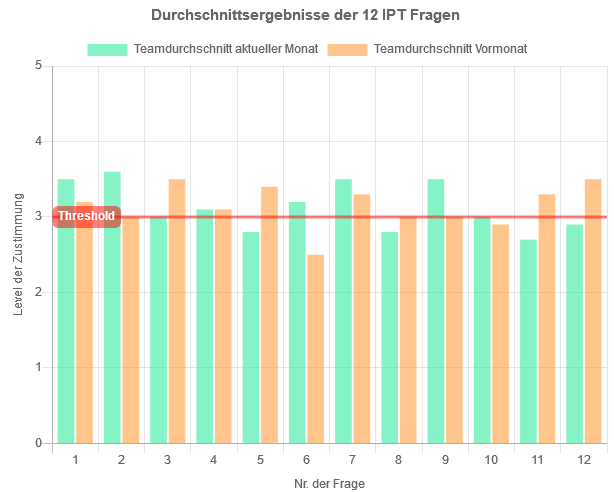
\includegraphics[width=0.7\textwidth]{picture.png}
\caption{Veranschaulichung der „threshold-Linie“.}
\end{figure}

\paragraph{}Das zweite Diagramm zeigt die Auswertung der letzten fünf Fragen im Fragebogen, welche sich allesamt auf die Teamleitung beziehen: Hier wird in einem Balkendiagramm die Einschätzung der Führungskräfte mit der Einschätzung des Rests des Teams verglichen, um mögliche Diskrepanzen aufzudecken, sodass den Managern nötige Handlungsfelder aufgezeigt werden. Das Diagramm wird zu Programmstart mit den entsprechenden Daten aus den bereitgestellten Funktionen bestückt und während der Laufzeit nicht weiter aktualisiert. Auch hier werden mit callbacks Kurzversionen der Fragen per mouseover eingeblendet.
Im dritten Diagramm werden mittels eines Liniendiagramms die Durchschnittsergebnisse der Stimmung im Team über die letzten 12 Umfragen angezeigt. Das Diagramm wird zu Programmstart mit den entsprechenden Daten aus den bereitgestellten Funktionen bestückt und während der Laufzeit nicht weiter aktualisiert. Es dient dazu, den Verlauf der Stimmung über längere Zeit einzufangen, und gegebenenfalls positive oder negative Trends zu erkennen.


Die weiteren verwendeten Optionen der Diagramme (Padding, Anzeigen von Labels und Legenden, Schrittweiten der Diagramme, …) sind dem Programmcode zu entnehmen.
Wichtig ist anzumerken, dass der Parameter „responsive“ auf „false“ gesetzt wurde, sodass die Diagramme beim Zoomen im Browser nicht mit skalieren, um eine sinnvolle Anzeige auf allen Displaygrößen zu gewährleisten (da bei sehr kleinen Bildschirmen Teile des Diagramms ohne Zoom nicht zu lesen waren).

Im letzten Teil des Plugins findet sich eine Tabelle zur Auswertung der Freitextantworten mittels NLP. Hierbei wird pro Monat dargestellt, welchen Anteil die 3 Kategorien (siehe 5.3) an den gesamten Beantwortungen haben. Somit lässt sich im Zeitverlauf gegebenenfalls eine Verbesserung/Verschlechterung der Stimmung ablesen. Besonders spannend ist, die Stimmung aus der NLP Tabelle mit der Stimmung im dritten Chart (Stimmung auf Skala von 1 bis 10) zu vergleichen. Rückschlüsse auf einzelne Mitarbeiter sind nicht möglich, da die Daten nur aggregiert dargestellt werden.

\paragraph{}Die notwendigen Änderungen im CSS-Style wurden direkt im gadget.xml file vorgenommen, um den Transfer der Dateien übersichtlich und kompakt zu halten. Eine Einbindung in den CSS Ordner hätte außerdem eine zusäzliche Änderung im atlassian-plugin.xml file bedingt. Daher wurde es der Einfachheit halber in den HTML Teil integriert.

\subsection{Testfälle}
Im Folgenden sollen einige Testfälle beispielhaft betrachtet werden.
\paragraph{i. Was passiert wenn mehr/weniger als 12 CSVs mit monatlichen Umfragedaten bereitliegen?}
Dieser Testfall betrifft das dritte Diagramm (Verlauf des Wohlbefindens im Team über 12 Monate)
Liegen mehr als 12 CSV Dateien vor, werden auf den Bottle Server nur die letzten 12 gelegt. In Jira werden dann freilich auch nur diese angezeigt. 
Liegen weniger als 12 vor, werden alle auf den Bottle Server gelegt. In Jira werden im Diagramm auf der X-Achse die letzten 12 Monate beschriftet, und die Balken laden für alle Monate, in denen auch Daten vorliegen. Im folgenden Screenshot ist der Fall dargestellt, dass es nur Daten für 4 Monate gibt:

\paragraph{ii. Was passiert wenn ein Mitarbeiter nicht alle Felder des Fragebogens ausfüllt?}
Die erste Frage sowie die folgenden 12 im Fragebogen sind Pflichtfragen. Im online Umfragetool wird sichergestellt, dass der Fragebogen nicht abgeschickt werden kann, falls hierfür keine Antwort abgegeben wird.
Die Frage zur Stimmung auf einer Skala von 1 bis 10 ist keine Pflichtfrage. Falls hier keine Antwort abgegeben wird, wird dies für die Berechnung des Durchschnitts im Javascript Code durch die Variable \emph{answerCounter} berücksichtigt. 
Die 3 Freitextfragen sind ebenfalls optional. Falls der Mitarbeiter hier nichts einträgt, wird ein NLP Score von 0 (=neutrale Stimmung) vergeben.

\paragraph{iii. Was passiert, wenn eine falsche Rolle (Mitarbeiter/Führungskraft) im Fragebogen angegeben wird?}
Die erste Frage im Fragebogen fragt, ob der Beantwortende eine Führungskraft oder ein "normaler"  Mitarbeiter ist.
Diese Unterscheidung ist für das zweite Chart wichtig. Falls hier jemand eine falsche Angabe macht, kann das System dies nicht korrigieren. Wir haben uns trotzdem für diese Umsetzung entschlossen, da man unserem Verständnis nach aus Jira nicht die Rolle eines Mitarbeiters zuverlässig erkennen kann. Es gibt zwar die Möglichkeit, zu erkennen ob ein jemand ein Admin ist, aber eine Führungskraft muss nicht zwangsweise ein Admin sein und umgekehrt. Daher haben wir vereinfachend angenonmmen, dass die Umfrageteilnehmer ihre Rolle wahrheitsgemäß angeben. Sicherlich sollte man dies in der Praxis nicht so umsetzen, jedoch erachten wir diese Vereinfachung im Rahmen des Praktikums als angemessen.

\paragraph{iv. Können in irgendeiner Form Rückschlüsse auf einzelne Mitarbeiter gezogen werden?}
Nein, denn es werden im Jira Dashboard lediglich Daten aus den CSVs von umfrageonline.com verarbeitet und dargestellt. Diese enthalten keinerlei Informationen wie etwa Namen oder Personalnummern, sodass nicht einmal aus den Rohdaten des Fragebogens herausgelesen werden kann, wer der Beantwortende war. Zudem werden alle Darstellungen auf Teamebene vollzogen.
\begin{figure}[htb]
\centering
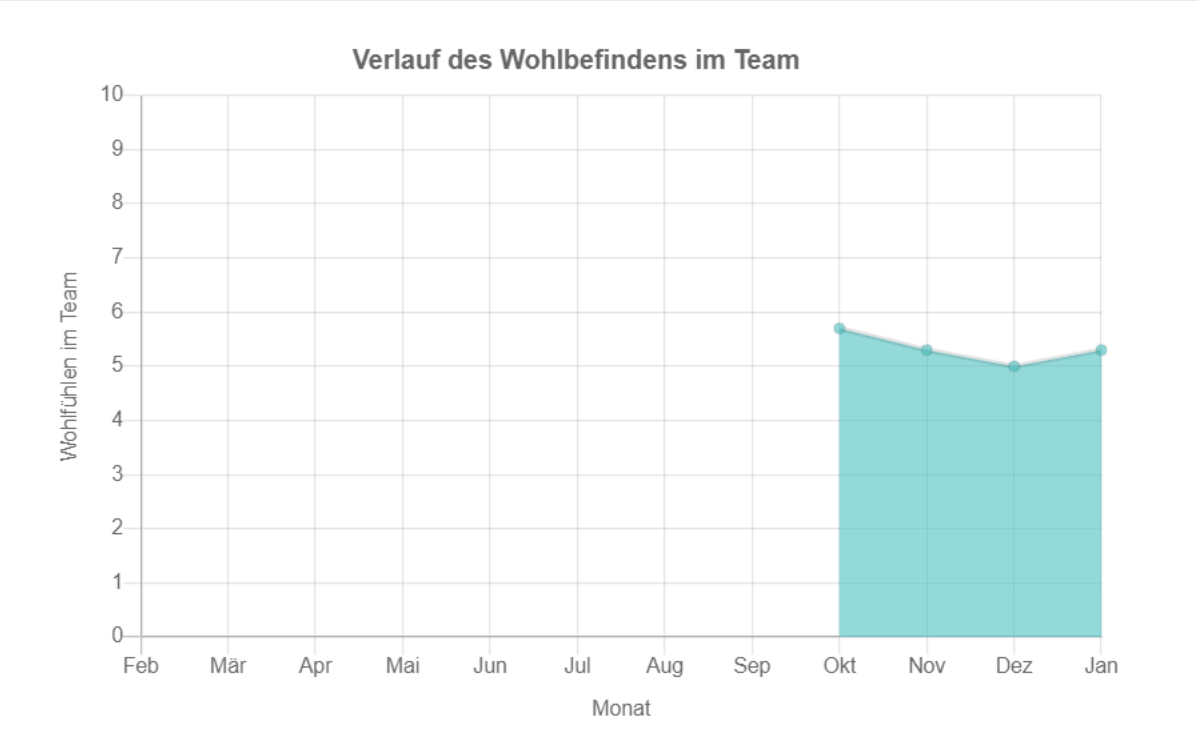
\includegraphics[width=0.7\textwidth]{picture2.png}
\caption{nur Umfragedaten von 4 Monaten verfügbar.}
\end{figure}


\end{document}

